\documentclass[]{report}

\voffset=-1.5cm
\oddsidemargin=0.0cm
\textwidth = 480pt

\usepackage{framed}
\usepackage{subfiles}
\usepackage{graphics}
\usepackage{newlfont}
\usepackage{eurosym}
\usepackage{amsmath,amsthm,amsfonts}
\usepackage{amsmath}
\usepackage{color}
\usepackage{amssymb}
\usepackage{multicol}
\usepackage[dvipsnames]{xcolor}
\usepackage{graphicx}
\begin{document}


HibColl Videos

%% --------------------%% --------------------%% --------------------%% --------------------%% ------------------------

1.A  Converting from Decimal to Binary
1.B  Converting from Decimal to Hexadecimal
1.C  Converting from Binary to Decimal
1.D  Converting from Hexadecimal to Decimal
1.E  Binary Addition
1.F  Binary Subtraction

%% --------------------%% --------------------%% --------------------%% --------------------%% ------------------------

2.A  Membership Tables
2.B  Venn Diagrams
2.C  Set differences and symmetric difference
2.D  
2.E



\chapter{Section 1}
\subsection{Significant Digits}
There are three rules on determining how many significant figures are in a number: Non-zero digits are always significant. Any zeros between two significant digits are significant. A final zero or trailing zeros in the decimal portion ONLY are significant.

\section{Floating Point Notation}



In computing, floating point describes a method of 
representing an approximation of a real number in a 
way that can support a wide range of values. 


The numbers are, in general, represented approximately 
to a fixed number of significant digits (the mantissa) and scaled using an exponent. 

In essence, computers are integer machines and are capable of representing real numbers only by using complex codes. The most popular code for representing real numbers is called the IEEE Floating-Point Standard .
The term floating point is derived from the fact that there is no fixed number of digits before and after the decimal point; that is, the decimal point can float. There are also representations in 
which the number of digits before and after the decimal point is set, called fixed-point representations. In general, floating-point representations are slower and less accurate than fixed-point representations, but they can handle a larger range of numbers.



\chapter{Set Theory}



\subsection{Cartesian Product}
{
\begin{itemize}
\item Let $X$ and $Y$ be sets.
\item The \textbf{cartesian product} $X \times Y$ is the set whose elements are \textbf{all} of 
the ordered pairs of elements $(x,y)$ where $x \in X$ and $y \in Y$.
\end{itemize}

\begin{itemize}
\item Let $X = \{a,b,c\}$
\item Let $Y = \{0,1\}$ 
\item The cartesian product $X \times Y$ is therefore:
\end{itemize}

\begin{itemize}
\item Importantly $X \times Y \neq Y \times X$
\item Recall: Let $X = \{a,b,c\}$ and let $Y = \{0,1\}$ 
\item The cartesian product $Y \times X$ is therefore:
\end{itemize}
}


%% --------------------%% --------------------%% --------------------%% --------------------%% ------------------------

3.3.A

4.4.B Logarithms
4.4.C 

%% --------------------%% --------------------%% --------------------%% --------------------%% ------------------------

5.2.A Graph Theory
5.2.B
%% --------------------%% --------------------%% --------------------%% --------------------%% ------------------------





\Large
\begin{center}
  \textbf{Number Systems - Tutorial Sheet 2}
\end{center}
\section*{Part A: Number Systems - Binary Numbers}
\begin{enumerate}
\item Express the following decimal numbers as binary numbers.
  \begin{multicols}{4}
    \begin{itemize}
    \item[i)] $(73)_{10}$
    \item[ii)] $(15)_{10}$
    \item[iii)] $(22)_{10}$
    \end{itemize}
  \end{multicols}

  All three answers are among the following options.
  \begin{multicols}{4}
    \begin{itemize}
    \item[a)] $(10110)_{2}$ %22
    \item[b)] $(1111)_{2}$ %15
    \item[c)] $(1001001)_{2}$ %73
    \item[d)] $(1000010)_{2}$ %64
    \end{itemize}
  \end{multicols}

\item Express the following binary numbers as decimal numbers.
  \begin{multicols}{4}
    \begin{itemize}
    \item[a)] $(101010)_{2}$
    \item[b)] $(10101)_{2}$
    \item[c)] $(111010)_{2}$
    \item[d)] $(11010)_{2}$
    \end{itemize}
  \end{multicols}
  \item Express the following binary numbers as decimal numbers.
  \begin{multicols}{4}
    \begin{itemize}
    \item[a)] $(110.10101)_{2}$
    \item[b)] $(101.0111)_{2}$
    \item[c)] $(111.01)_{2}$
    \item[d)] $(110.1101)_{2}$
    \end{itemize}
  \end{multicols}
\item Express the following decimal numbers as binary numbers.
  \begin{multicols}{4}
    \begin{itemize}
    \item[a)] $(27.4375)_{10}$  %
    \item[b)] $(5.625)_{10}$
    \item[c)] $(13.125)_{10}$
    \item[d)] $(11.1875)_{10}$
    \end{itemize}
  \end{multicols}
\end{enumerate}
\newpage
\section*{Part B: Number Systems - Binary Arithmetic}
%http://www.csgnetwork.com/binaddsubcalc.html
%(See section 1.1.3 of the text)
\begin{enumerate}
\item Perform the following binary additions.
  \begin{multicols}{2}
    \begin{itemize}
    \item[a)] $(110101)_{2}$ + $(1010111)_{2}$
    \item[b)] $(1010101)_{2}$ + $(101010)_{2}$
    \item[c)] $(11001010)_{2}$ + $(10110101)_{2}$
    \item[d)] $(1011001)_{2}$ + $(111010)_{2}$
    \end{itemize}
  \end{multicols}

\item Perform the following binary subtractions.
  \begin{multicols}{2}
    \begin{itemize}
    \item[a)] $(110101)_{2}$ - $(1010111)_{2}$
    \item[b)] $(1010101)_{2}$ - $(101010)_{2}$
    \item[c)] $(11001010)_{2}$ - $(10110101)_{2}$
    \item[d)] $(1011001)_{2}$ - $(111010)_{2}$
    \end{itemize}
  \end{multicols}


\item Perform the following binary multiplications.
\begin{multicols}{2}
\begin{itemize}
\item[a)] $(1001)_{2}\times( 1000)_{2}$  % 9 by 8
\item[b)] $(101)_{2}\times(1101)_{2}$ % 5 by 11
\item[c)] $(111)_{2}\times(1111)_{2}$ % 7 by 15
\item[d)] $(10000)_{2}\times(11001)_{2}$    %16 by 25
\end{itemize}
 \end{multicols}



\item Perform the following binary multiplications.
%\begin{multicols}{2}
%\begin{itemize}
%\item[a)] $(1001000)_{2} \div ( 1000)_{2}$
%\item[b)] $(101101)_{2} \div (1001)_{2}$
%\item[c)] $(1001011000)_{2} \div (101000)_{2}$
%\item[d)] $(1100000)_{2} \div (10000)_{2}$
%\end{itemize}
%\end{multicols}

\begin{enumerate}
\item Which of the following binary numbers is the result of this binary division: $(10)_{2} \times ( 1101)_{2}$. % % (2) /  (13)
\begin{multicols}{2}
\begin{itemize}
\item[a)] $(11010)_{2}$ %26
\item[b)] $(11100)_{2}$ %28
\item[c)] $(10101)_{2}$ %21
\item[d)] $(11011)_2$ %27
\end{itemize}
\end{multicols}
\item Which of the following binary numbers is the result of this binary division: $(101010)_{2} \times( 111 )_{2}$. % (4) /  (6)
\begin{multicols}{2}
\begin{itemize}
\item[a)] $(11000)_{2}$ %24
\item[b)] $(11001)_{2}$ %25
\item[c)] $(10101)_{2}$ %21
\item[d)] $(11011)_2$ %27
\end{itemize}
\end{multicols}
\item Which of the following binary numbers is the result of this binary division: $(1001110)_{2}\times ( 1101 )_{2}$. % (9) /  (3)
\begin{multicols}{2}
\begin{itemize}
\item[a)] $(11000)_{2}$ %24
\item[b)] $(11001)_{2}$ %25
\item[c)] $(10101)_{2}$ %21
\item[d)] $(11011)_2$ %27
\end{itemize}
\end{multicols}
\end{enumerate}

%----------------------------------------------------------------%

\item Perform the following binary divisions.
%\begin{multicols}{2}
%\begin{itemize}
%\item[a)] $(1001000)_{2} \div ( 1000)_{2}$
%\item[b)] $(101101)_{2} \div (1001)_{2}$
%\item[c)] $(1001011000)_{2} \div (101000)_{2}$
%\item[d)] $(1100000)_{2} \div (10000)_{2}$
%\end{itemize}
%\end{multicols}

\begin{enumerate}
\item Which of the following binary numbers is the result of this binary division: $(111001)_{2} \div ( 10011)_{2}$. % (57) /  (19)
\begin{multicols}{2}
\begin{itemize}
\item[a)] $(10)_2$ %2
\item[b)] $(11)_{2}$ %3
\item[c)] $(100)_{2}$ %4
\item[d)] $(101)_{2}$ %5
\end{itemize}
\end{multicols}
\item Which of the following binary numbers is the result of this binary division: $(101010)_{2} \div ( 111 )_{2}$. % (42) /  (7)
\begin{multicols}{2}
\begin{itemize}
\item[a)] $(11)_2$ %3
\item[b)] $(100)_{2}$ %4
\item[c)] $(101)_{2}$ %5
\item[d)] $(110)_{2}$ %6
\end{itemize}
\end{multicols}
\item Which of the following binary numbers is the result of this binary division: $(1001110)_{2} \div ( 1101 )_{2}$. % (78) /  (13)
\begin{multicols}{2}
\begin{itemize}

\item[a)] $(100)_{2}$ %4
\item[b)] $(110)_{2}$ %6
\item[c)] $(111)_{2}$ %7
\item[d)] $(1001)_2$ %9
\end{itemize}
\end{multicols}
\end{enumerate}


\end{enumerate}

\newpage
\section*{Part C: Number Bases - Hexadecimal}
\begin{enumerate}

\item Answer the following questions about the hexadecimal number systems
\begin{itemize}
\item[a)] How many characters are used in the hexadecimal system?
\item[b)] What is highest hexadecimal number that can be written with two characters? \item[c)] What is the equivalent number in decimal form?
\item[d)] What is the next highest hexadecimal number?
\end{itemize}


\item Which of the following are not valid hexadecimal numbers?
  \begin{multicols}{4}
    \begin{itemize}
    \item[a)] $73$
    \item[b)] $A5G$
    \item[c)] $11011$
    \item[d)] $EEF	$
    \end{itemize}
  \end{multicols}

\item Express the following decimal numbers as a hexadecimal number.
  \begin{multicols}{4}
    \begin{itemize}
    \item[a)] $(73)_{10}$
    \item[b)] $(15)_{10}$
    \item[c)] $(22)_{10}$
    \item[d)] $(121)_{10}$
    \end{itemize}
  \end{multicols}


\item Compute the following hexadecimal calculations.
  \begin{multicols}{4}
    \begin{itemize}
    \item[a)] $5D2+A30$
    \item[b)] $702+ABA$
    \item[c)] $101+111$
    \item[d)] $210+2A1$
    \end{itemize}
  \end{multicols}
\end{enumerate}


\newpage





% \newpage
\section*{Part D: Natural, Rational and Real Numbers}
\begin{framed}
\begin{itemize}
\item $\mb{N}$ : natural numbers (or positive integers) $\{1,2,3,\ldots\}$
\item $\mb{Z}$ : integers $\{-3,-2,-1,0,1,2,3,\ldots\}$
\begin{itemize}
\item[$\ast$] (The letter $\mb{Z}$ comes from the word \emph{Zahlen} which means ``numbers" in German.)
\end{itemize}
\item $\mb{Q}$ : rational numbers
\item $\mb{R}$ : real numbers
\item $\mb{N} \subseteq \mb{Z } \subseteq \mb{Q} \subseteq \mb{R}$
\begin{itemize}
\item[$\ast$] (All natural numbers are integers. All integers are rational numbers. All rational numbers are real numbers.)
\end{itemize}
\end{itemize}
\end{framed}

\begin{enumerate}
\item State which of the following sets the following numbers belong to. 
  \begin{multicols}{4}
    \begin{itemize}
    \item[1)] $18$
    \item[2)] $8.2347\ldots$
    \item[3)] $\pi$
    \item[4)] $1.33333\ldots$
    \item[5)] $17/4$
    \item[6)] $4.25$
    \item[7)] $\sqrt{\pi}$
    \item[8)] $\sqrt{25}$
    %\item[i)]
    %\item[j)] $(15)_{10}$
    %\item[k)] $\pi$
    %\item[l)] $11.132$
    \end{itemize}
  \end{multicols}
  \bigskip
  The possible answers are

    \begin{itemize}
    \item[a)] Natural number : $\mb{N} \subseteq \mb{Z } \subseteq \mb{Q} \subseteq \mb{R}$
    \item[b)] Integer : $ \mb{Z } \subseteq \mb{Q} \subseteq \mb{R}$
    \item[c)] Rational Number : $ \mb{Q} \subseteq \mb{R}$
    \item[d)] Real Number $\mb{R}$

    %\item[i)]
    %\item[j)] $(15)_{10}$
    %\item[k)] $\pi$
    %\item[l)] $11.132$
    \end{itemize}

\end{enumerate}



\end{document}

% \item The Fibonacci sequence $f_n$ is defined recursively by the rule
%   \begin{equation*}
%     \begin{cases}
%       f_0&=0\\
%       f_1&=1\\
%       f_n&=a_{n-1}+a_{n-2}
%     \end{cases}
%   \end{equation*}

%   \begin{enumerate}
%   \item
%     Write a program to evaluate the Fibonacci sequence and hence evaluate $f_{50}$.
%   \item
%     Let the sequence $g_n$ be defined as the ratio
%     \begin{equation*}
%       g_n = \frac{f_{n+1}}{f_n}
%     \end{equation*}
%     Write a program to evaluate the first $50$ terms of the sequence $g_n$.
%   \item
%     Assumming that the sequence $g_n$ has a limit $\phi$, find this limit.
%   \end{enumerate}





\subsection{The Cartesian Product}
Exercises


 Discrete Maths
 
A binary relation on a set A is the collection of ordered pairs of elements of A. In other words, it is the subset of the cartesian product A2= AA

Cartesian Product
 
This is a direct product pf 2 sets
 
XY = {(x,y)| xXandyY }
 
4 suits of cards and 13 Ranks, therefore 52 element cartesian prodcut.
 
N.B         AB BA
              A=A =
 
Cartesian product is not associative
\chapter{graph theory }
Given the following definitions for simple, connected graphs:
\begin{itemize}
\item $K_n$ is a graph on $n$ vertices where each pair of vertices is connected by an edge;
\item $C_n$ is the graph with vertices $v_1, v_2, v_3, \dots, v_n$ and edges $\{v_1,v_2\}, \{v_2,v_3\}, \dots\{v_n, v_1\}$;
\item $W_n$ is the graph obtained from $C_n$ by adding an extra vertex,$v_{n+1}$, and edges
from this to each of the original vertices in $C_n$.
\end{itemize}
(a) Draw $K_4$, $C_4$, and $W_4$. 
%%% --------------------%% --------------------%% --------------------%% --------------------%% --------------------%% --------------------%% --------------------%% --------------------%% --------------------%% ------------------------%

\section{Set Theory}
\begin{enumerate}
\item The Universal Set $\mathcal{U}$
\item Union
\item Intersection
\item Set Difference
\item Relative Difference
\end{enumerate}


%---------------------------------------%
\newpage

Question 2B 2010 Zone A


\begin{itemize}
	\item Let A and B be subsets of the a universal set $U$.
	\item Use membership tables to prove that $(A \cup B^{\prime})^{\prime}$ = $A^{\prime} \cap B$
	\item Shade the regions corresponding to this set on a Venn Diagram
\end{itemize}

\begin{tabular}{|c|c|| c | c| c|}
	A	&	B	&	$B^{\prime}$	&	$A \cup B^{\prime}$	&	$(A \cup B^{\prime})^{\prime}$	\\ \hline
	0	&	0	&	1	&	1	&	0	\\
	0	&	1	&	0	&	0	&	1	\\
	1	&	0	&	1	&	1	&	0	\\
	1	&	1	&	0	&	1	&	0	\\
\end{tabular}									

\begin{tabular}{|c|c|| c | c| }									
	A	&	B	&	$A^{\prime}$	&	$A^{\prime} \cap B$	\\	\hline	
	0	&	0	&	1	&	0	\\		
	0	&	1	&	1	&	1	\\		
	1	&	0	&	0	&	0	\\		
	1	&	1	&	0	&	0	\\		
\end{tabular}



%-------------------------------------------%
% 2010 Zone A Q 1c
Given the universal set $U$ and subsets $A$ and $B$, list the set $(A \cup B^{\prime})^{\prime}$
\begin{itemize}
	\item $U=\{1,2,\ldots,8,9\}$
	\item $A=\{2,4,6,8\}$
	\item $B=\{ 4,5,6,7\}$
	\item $B^{\prime}=\{ 1, 2, 3, 8, 9  \}$
	\item $A \cup B^{\prime}=\{ 1, 2, 3,4, 6, 8, 9  \}$
	\item $(A \cup B^{\prime})^{\prime}=\{ 5,7 \}$
\end{itemize}


\newpage

%----------------------------------------------------------------%

\subsection{Number Sets}

%% \vspace{-1cm}
\textbf{Blackboard Bold Typeface}

\begin{itemize}
\item Conventionally the symbols for numbers sets are written in a special typeface, known as \textbf{blackboard bold}.
\item Examples : $\mathbb{N}$, $\mathbb{Z}$ and $\mathbb{R}$.

\end{itemize}

%----------------------------------------------------------------%

\subsection{Number Sets}

%% \vspace{-1cm}
\textbf{Natural Numbers} ($\mathbb{N}$)
\begin{itemize}
\item The whole numbers from 1 upwards. 

\item The set of natural numbers is 
\[\{1,2,3,4,5,6,\ldots\} \]
\item In some branches of mathematics, $0$ might be counted as a natural number.
\[\{0,1,2,3,4,5,6,\ldots\} \]
\end{itemize}
 
%----------------------------------------------------------------%

 
 \subsection{Number Sets}
 
 
 %% \vspace{-0.5cm}
 \textbf{Integers} ($\mathbb{Z}$)
 \begin{itemize}
 \item The integers are all the whole numbers, all the negative whole numbers and zero.
 
 \item The set of integers is 
 \[\{\ldots,-4,-3,-2,-1,\;0,\;1,\;2,\;3,\ldots\} \]
 \item The notation $\mathbb{Z}$ is from the German word for numbers: \textit{Zahlen}. 
 \item All natural numbers are integers.
 \[ \mathbb{Q}  \subset \mathbb{Z}\]
 \end{itemize}
  
 %----------------------------------------------------------------%
 
  
  \subsection{Number Sets}
    
  %% \vspace{-1.8cm}
  \textbf{Integers} ($\mathbb{Z}$)
  \begin{itemize}
 \item Natural numbers may also be referred to as positive integers, denoted $\mathbb{Z}^{+}$. \\(note the superscript)
 \item Negative integers are denoted $\mathbb{Z}^{-}$.
 \[\{\ldots,-4,-3,-2,-1\}\]
  \end{itemize}
   
  %----------------------------------------------------------------%
  
   
   \subsection{Number Sets}
     
   %% \vspace{-1.8cm}
   \textbf{Integers} ($\mathbb{Z}$)
   \begin{itemize}
 \item 0 is neither positive nor negative. The following set of non-negative numbers \[\{0,1,2,3,4,5,6,\ldots\} \] might be denoted $0 \cup \mathbb{Z}^{+}$
 \item $\cup$ is the mathematical symbol for \textbf{union}.
 \end{itemize}
  


\subsection{Number Sets}

%% \vspace{-1cm}
\textbf{Rational Numbers} ($\mathbb{Q}$)
\begin{itemize}
\item Rational numbers, also known as quotients, are numbers you can make by dividing one integer by another (but not dividing by zero). 
\item If a number can be expressed as one integer divided by another, it is a rational number.
\[ \mathbb{Q} = \left\{\; \frac{p}{q} \;\bigg| p \in \mathbb{Z},\; q \in \mathbb{Z},\; q \neq 0  \;   \right\}   \]
\end{itemize}

%-------------------------------------------------------------- %   

\subsection{Number Sets}

%% \vspace{-1cm}
\textbf{Rational Numbers} ($\mathbb{Q}$)
   \begin{itemize}
   \item All integers are rational numbers 
   \[ \mathbb{Z}  \subset \mathbb{Q}\]
   (and by extension all natural numbers are rational numbers too)
   \item Examples of rational numbers
   \[ 9500,\;7,\; \frac{1}{2} ,\; \frac{3}{7},\; -2.6 ,\; 0.001\] 
   \end{itemize}
   
   %-------------------------------------------------------------- %   
   
   \subsection{Number Sets}
   
   %% \vspace{-1cm}
   \textbf{Irrational Numbers} 
      \begin{itemize}
   \item A number that can not be written as the ratio of two integers is known as an irrational number.
   \item Two famous examples of irrational numbers are $\pi$ and $\sqrt{2}$. 
   \[\pi = 3.141592\ldots\]
   \[\sqrt{2} = 1.41421\ldots\]
   \end{itemize}
    

\subsection{Number Sets}

%% \vspace{-1cm}
\textbf{Real Numbers} ($\mathbb{R}$)
\begin{itemize}
\item Irrational numbers are types of real numbers.
\item Rational numbers are real numbers too.
\[ \mathbb{Q}  \subset \mathbb{R}\]

\item A real number is simply any point anywhere on the number line.
   \end{itemize}
    

\subsection{Number Sets}

%% \vspace{-1cm}
\textbf{Real Numbers} ($\mathbb{R}$)
\begin{itemize}
\item There are numbers that are not real numbers, for example \textbf{imaginary numbers}, but we will not cover them in this presentation.
\end{itemize}

   
%------------------------------------------$
2010 Zone B Q 1

5n+1 Rules of Inclusion method

$A = \{5n+1: n \in Z \}$
\subsection*{Floating Point Notation}
(Demonstration on white board)

\subsection*{2011 Zone A question 1d}

Showing your workings, express the repeating decimal 0.012012012012...
as a rational number in its simplest form.


\begin{itemize}
\item x = 0.012012012012...
\item 10x = 0.12012012012... (not particularly useful )
\item 100x = 1.2012012012... (not particularly useful either)
\item 1000x= 12.012012012... (very useful)
\item 999x = 12
\item x= 12/999 = 4/333 (Answer!)
\end{itemize}

%------------------------------------------$

\subsection*{2008  Zone A question2a}
$B = \{3n-1 :n \in Z^{+} \}$
Describe the set B using the listing method

\begin{itemize}
	\item Let $n=1$. Consequently $3(1)-1 =2$
	\item Let $n=2$. Likewise $3(2)-1 =5$
	\item Let $n=3$. $3(3)-1 = 8 $
	\item The repeated differences are 3. The next few values are 11, 14 and 17
	\item So by the listing method $B= \{2,5,8,11,14,17,\ldots\}$
\end{itemize}

$A = \{3,5,7,9,ldots \}$
Describe the set A using the rules of inclusion method

\begin{itemize}
	\item The repeated differences are 2.
	\item We can say the rule has the form $2n+k$
	\item For the first value n=1. Therefore $2+k=3$
	\item Checking this , for the second value , n=2. Therefore $4+k=5$
	\item Clearly k = 1.
	\item $A = \{2n+1 :n \in Z^{+} \}$
	\item So by the listing method $B= \{2,5,8,11,14,17,\ldots\}$
\end{itemize}

\section{Set Theory}
\begin{enumerate}
	\item The Universal Set $\mathcal{U}$
	\item Union
	\item Intersection
	\item Set Difference
	\item Relative Difference
\end{enumerate}


Set theory

\subsection{Specifying Sets (2.1)}

\begin{enumerate}
\item Listing Method
\item Rules of Inclusion
\end{enumerate}

Subsets (2.2)
Subsets and Proper Subsets
Cardinality of a Set
Power Set


\subsection{Set operations (2.3)}

complement
union 
intersection
set difference


venn diagrams
8 Disjoint Regions

DE Muorgan's Laws (Useful for Propositions)

membership tables

proof by truth tables
AND
OR
NOT
Set difference
symmetric difference



\newpage


Harmonic Mean

\[ H_x = \frac{ n }{ \frac{ 1 }{ x_1 } + \frac{ 1 }{ x_2 } + \cdots + \frac{ 1 }{ x_n } } \]

2,4,6,8
> 1/mean(1/a)
[1] 3.84
> 1/a
[1] 0.5000000 0.2500000 0.1666667 0.1250000
> sum(1/a)
[1] 1.041667
> sum(1/a)*24
[1] 25
> 96/25
[1] 3.84



\subsection{Functions}
Consider the floor function $f : R \rightarrow Z$ given the rule

\[ f(x) = \lfloor \frac{x+1}{2} \rfloor \]

\begin{enumerate}
\item evaluate $f(6)$ and $f(-6)$
\item Show that f(x) is not one-to-one
\item 
\end{enumerate}

%----------------------------------------%

\subsection{Functions}
Evaluate $f(6)$ 


\[ f(x) = \lfloor \frac{x+1}{2} \rfloor \]


\[ f(6) = \lfloor \frac{\boldsymbol{6}+1}{2}\rfloor = \lfloor  \frac{7}{2}\rfloor\]


\[  \lfloor 3.5 \rfloor  = 3  \]


%----------------------------------------%

\subsection{Functions}
Evaluate $f(-6)$ 


\[ f(x) = \lfloor \frac{x+1}{2} \rfloor \]


\[ f(6) = \lfloor \frac{\boldsymbol{-6}+1}{2}\rfloor = \lfloor  \frac{-5}{2}\rfloor\]


\[  \lfloor -2.5 \rfloor  = -3  \]






% http://www.textbooksonline.tn.nic.in/books/12/std12-bm-em-1.pdf


\subsection{Discrete Maths : Relations}

\begin{itemize}
\item A relation $R$ from a set A to a set B is a subset of the
\textbf{cartesian product} A x B. 
\item Thus R is a set of \textbf{ordered pairs} where
the first element comes from A and the second element comes
from B i.e. $(a, b)$
\end{itemize}

%-----------------------------------%

\subsection{Discrete Maths : Relations}

\begin{itemize}

\item  If $(a, b) \in R$ we say that $a$ is related to $b$ and write $aRb$.
\item If $(a, b) \notin R$, we say that $a$ is not related to $b$ and write $aRb$. CHECK
\item If
$R$ is a relation from a set $A$ to itself then we say that ``$R$ is a relation
on $A$".
\end{itemize}

%-----------------------------------%

\subsection{Discrete Maths : Relations}

%% \vspace{-2cm}
\textbf{Example}
\begin{itemize}
\item Let $A = \{2, 3, 4, 6\}$ and $B = \{4, 6, 9\}$
\item Let R be the relation from A to B defined by \textit{\textbf{xRy}} if $x$
divides $y$ exactly.
\end{itemize}


%-----------------------------------%

\subsection{Discrete Maths : Relations}

%% \vspace{-0.7cm}
\textbf{Example}
\begin{itemize}

\item Let $A = \{2, 3, 4, 6\}$ and $B = \{4, 6, 9\}$
\item Let R be the relation from A to B defined by \textit{\textbf{xRy}} if $x$
divides $y$ exactly.
\item  Then
\[R = {(2, 4), (2, 6), (3, 6), (3, 9), (4, 4), (6, 6)}\]
\end{itemize}



%----------------------------------------%
\chapter{Logic}

%--------------------------------------%

\section{Logic Proposition}
Let $p$, $Q$ and $r$ be the following propositions concerning integers $n$:

\begin{itemize}
\item $p$ : n is a factor of 36 (2)
\item $q$ : n is a factor of 4 (2)
\item $r$ : n is a factor of 9 (3)
\end{itemize}

{

\begin{center}
\begin{tabular}{|c||c|c|c|}
\hline 
\phantom{spa} \textbf{n} \phantom{spa}	& \phantom{spa}	\textbf{p} \phantom{spa}	& \phantom{spa}	\textbf{q} \phantom{spa}	& \phantom{spa}	\textbf{r} \phantom{spa}	\\ \hline \hline
1	&	1	&	1	&	1	\\ \hline
2	&	1	&	0	&	1	\\ \hline
3	&	0	&	1	&	1	\\ \hline
4	&	1	&	0	&	1	\\ \hline
6	&	0	&	0	&	1	\\ \hline
9	&	0	&	1	&	1	\\ \hline
12	&	0	&	0	&	1	\\ \hline
18	&	0	&	0	&	1	\\ \hline
36	&	0	&	0	&	1	\\
\hline 
\end{tabular} 
\end{center}
}
For each of the following compound statements, express it using the propositions P q and r, andng logical symbols, then given the truth table for it,

\begin{itemize}
\item[1)] If n is a factor of 36, then n is a factor of 4 or n is a factor of 9
\item[2)] If n is a factor of 4 or n is a factor of 9 then  n is a factor of 36
\end{itemize}

%--------------------------------------%

\newpage

\section*{Part 1 : Logic}


\subsection*{1.1 2010 Question 3}
Let $S = \{10,11,12,13,14,15,16,17,18,19\}$ and let p, q be the following propositions concerning the integer $n \in S$.

\begin{itemize}
\item p: n is a multiple of two. (i.,18e. $\{10,12,14,16,18\}$)
\item q: n is a multiple of three. {i.e. $\{12,15,18\}$}
\end{itemize}

For each of the following compound statements find the sets of values n for which it is true. 

\begin{itemize}
\item $p \vee q$ : (p or q :  10 12 14 15 16 18) 
\item $p \wedge q$: (p and q: 12 18)
\item $ \neg p \oplus q$: (not-p or q, but not both)
\begin{itemize}
\item $\neg p $ not-p = $\{ 11 13 15 17 19\}$
\item $\neg p \vee q$ not-p or q $\{11 12 13 15 17 18 19\}$
\item $\neg p \wedge q$ not-p and q $\{15\} $
\item $ \neg p \oplus q$ = $\{11, 12, 13, 17, 18, 19\}$
\end{itemize}
\end{itemize}

%--------------------------------------------------- %

%--------------------------------------------------- %
\subsection*{1.2 2010 Question 3}

Let p and q be propositions. Use Truth Tables to prove that

\[ p \rightarrow q \equiv \neg q \rightarrow \neg\]
\textbf{Important} Remember to make a comment at the end to say why the table proves that the two statements are logically equivalent. e.g. \emph{‘since the columns are identical both sides of the equation are equivalent’}.
{ 
\begin{tabular}{|c|c||c|}
\hline  p&  q& $p \rightarrow q$ \\ 
\hline  0&  0&  1\\ 
\hline  0&  1&  1\\ 
\hline  1&  0&  0\\ 
\hline  1&  1&  1\\ 
\hline 
\end{tabular} \hspace{0.5cm} \begin{tabular}{|c|c||c|c|c|}
\hline  p&  q& $\neg q$ & $\neg p$ & $\neg q \rightarrow \neg p$ \\ 
\hline  0&  0& 1& 1& 1\\ 
\hline  0&  1& 0& 1& 1\\ 
\hline  1&  0& 1& 0& 0\\ 
\hline  1&  1& 0& 0& 1\\ 
\hline 
\end{tabular}
} 
(Key ``difference" is first and last rows)
%--------------------------------------------------- %
%--------------------------------------------------- %
\subsection*{1.3 Membership Tables for Laws}
\emph{Page 44 (Volume 1) Q8.
Also see Section 3.3 Laws of Logic.}\\

Construct a truth table for each of the following compound statement and hence find simpler propositions to which it is equivalent.


\begin{itemize}
\item $p \vee F$
\item $p \wedge T$
\end{itemize}
\textbf{Solutions}
\begin{center}
{
\begin{tabular}{|c|c||c|c|}
\hline  p & T & $p \vee T$ & $ p \wedge T$ \\ \hline
\hline  0 & 1 & 1 & 0 \\ 
\hline  1 &  1 & 1 & 1 \\ 
\hline 
\end{tabular} 
}
\end{center}
\begin{itemize}
\item Logical OR: $p \vee T = T $
\item Logical AND: $p \wedge T = p  $
\end{itemize}

%-------------------------------------%
\begin{center}
{
\begin{tabular}{|c|c||c|c|}
\hline  p & F & $p \vee F$ & $ p \wedge F$ \\ \hline
\hline  0 & 0 & 0 & 0 \\ 
\hline  1 &  0 & 1 & 0 \\ 
\hline 
\end{tabular} 
}
\end{center}
\begin{itemize}
\item Logical OR:  $p \vee F = p $
\item Logical AND: $p \wedge F = F $
\end{itemize}
%--------------------------------------------------- %
%--------------------------------------------------- %
\subsection*{1.4 Propositions}
\textbf{Page 67 Question 9}
Write the contrapositive of each of the following statements:

\begin{itemize}
\item If n= 12, then n is divisible by 3.
\item If n=5, then n is positive.
\item If the quadrilateral is square, then four sides are equal.
\end{itemize}

\textbf{Solutions}
\begin{itemize}
\item If n is not divisible by 3, then n is not equal to 12.
\item If n is not positive, then n is not equal to 5.
\item If the four sides are not equal, then the quadrilateral is not a square.
\end{itemize}


%--------------------------------------------------- %
%--------------------------------------------------- %
\subsection*{1.5 Truth Sets}
\textbf{2009} 

Let $n = \{1, 2,3,4, 5,6,7, 8, 9\}$ and let p, q be the following propositions concerning the integer $n$.
\begin{itemize}
\item p: n is even, 
\item q: $n\geq 5$.
\end{itemize}
By drawing up the appropriate truth table find the truth set for each of the
propositions $p \vee \neg q$ and $ \neg q \rightarrow p$

\begin{tabular}{|c|c|c|c|c|}
\hline n & p & q & $\neg q$ & $p \vee \neg q$ \\ 
\hline 1 & 0 & 0 & 1 & 1\\ 
\hline 2 & 1 & 0 & 1 & 0\\ 
\hline 3 & 0 & 0 & 1 & 1\\ 
\hline 4 & 1 & 0 & 1 & 0\\ 
\hline 5 & 0 & 1 & 0 & 1\\ 
\hline 6 & 1 & 1 & 0 & 1\\ 
\hline 7 & 0 & 1 & 0 & 1\\ 
\hline 8 & 1 & 1 & 0 & 1\\ 
\hline 9 & 0 & 1 & 0 & 1\\ 
\hline 
\end{tabular} 
\[\mbox{Truth Set} = \{1,3,5,6,7,8,9\}\]

\begin{tabular}{|c|c|c|c|c|}
\hline n & p & q & $  q \rightarrow p$ & $  q \rightarrow p$ \\ 
\hline 1 & 0 & 0 & 1 & 0\\ 
\hline 2 & 1 & 0 & 1 & 0\\ 
\hline 3 & 0 & 0 & 1 & 0\\ 
\hline 4 & 1 & 0 & 1 & 0\\ 
\hline 5 & 0 & 1 & 0 & 1\\ 
\hline 6 & 1 & 1 & 1 & 0\\ 
\hline 7 & 0 & 1 & 0 & 1\\ 
\hline 8 & 1 & 1 & 1 & 0\\ 
\hline 9 & 0 & 1 & 0 & 1\\ 
\hline 
\end{tabular} 
\[\mbox{Truth Set} = \{5,7,9\}\]
%---------------------------------------
%--------------------------------------------------- %
%--------------------------------------------------- %
\newpage
\subsection*{1.6 Biconditional}
\emph{See Section 3.2.1}.\\
Use truth tables to prove that $ \neg p \leftrightarrow \neg q $ is equivalent to  $ p \leftrightarrow q $

\begin{tabular}{|c|c|c|}
\hline  p& q & $p \leftrightarrow q$ \\ 
\hline  0& 0 &  1\\ 
\hline  0& 1 &  0\\ 
\hline  1& 0 &  0\\ 
\hline  1& 1 &  1\\ 
\hline 
\end{tabular} 


\begin{tabular}{|c|c|c|c|c|}
\hline  p& q & $\neg p$ & $\neg q$ & $p \leftrightarrow q$ \\ 
\hline  0& 0 & 1& 1 & 1\\ 
\hline  0& 1 &  1& 0& 0\\ 
\hline  1& 0 &  0& 1& 0\\ 
\hline  1& 1 &  0 & 0& 1\\ 
\hline 
\end{tabular} 
\newpage
%--------------------------------------------------- %
%--------------------------------------------------- %
\subsection*{1.7 2008 Q3b Logic Networks }

Construct a logic network that accepts as input p and q, which may independently have the value 0 or 1, and
gives as final input $\neg(p \wedge \not q)$ (i.e. $\equiv p \rightarrow q$).\\
\bigskip

\textbf{Logic Gates}
\begin{itemize}
\item AND
\item OR
\item NOT
\end{itemize}
\bigskip

\emph{\textbf{Examiner's Comments:}Many
diagrams were carefully and clearly drawn and well labelled, gaining full
marks. The logic table was also well done by most, but there were a few marks
lost in the final part by failing to deduce that ‘since the columns of the table are
identical the expressions are equivalent’.}

%--------------------------------------------------- %
%--------------------------------------------------- %
\subsection*{1.8 2008 Q3b Logic Networks }
Construct a logic network that accepts as input p and q, which may independently have the value 0 or 1, and
gives as final input $(p \wedge  q) \vee \neg q$ (i.e. $\equiv p \rightarrow q$).



\textbf{Important} Label each of the gates appropriately and label the diagram with a symblic expression for the output after each gate.

%----------------------------------------------------------- %
\newpage

\section*{Prepositional Logic}

\subsection{five basic connectives}


%--------------------------------------------------%
Reflexive, Symmetric and Transitive

\begin{itemize} 
\item Reflexive
\item Symmetric
\item Transitive
\end{itemize}

%--------------------------------------------------%
\subsection{Logarithms}


Here we
assume x and y are positive real numbers.
1. $loga(xy) = loga(x) + loga(y)$
2. $loga(x/y)= loga(x) - loga(y)$
3. $loga (x^r) = r loga(x)$ for any real number r.
%--------------------------------------------------%
Invertible Functions

%--------------------------------------------------%
\subsection{Proof by Induction}

Another sequence is defined by the recurrence relation un = un-1+2n-1 and
u1 = 1.
(i) Calculate u2, u3, u4 and u5.
1,4,9,16,25

(ii) Prove by induction that $u_n = n^2$ for all $n \geq 1$

%--------------------------------------------------%
Exponentials
% http://www.mathsisfun.com/algebra/exponent-laws.html

\section{Laws of Exponents}
Here are the Laws (explanations follow):

Law	Example
x1 = x	61 = 6
x0 = 1	70 = 1
x-1 = 1/x	4-1 = 1/4
xmxn = xm+n	x2x3 = x2+3 = x5
xm/xn = xm-n	x6/x2 = x6-2 = x4
(xm)n = xmn	(x2)3 = x2×3 = x6
(xy)n = xnyn	(xy)3 = x3y3
(x/y)n = xn/yn	(x/y)2 = x2 / y2
x-n = 1/xn	x-3 = 1/x3
%--------------------------------------------------%
Z Score
\[ Z = \frac{X - \mu}{\sigma} \]
%--------------------------------------------------%




%-------------------------------------------------------%


%% --------------------
\subsection{Exercises}

Showing your workings, use the rules of indices and logarithms to give the following two expression in their simplest form.
\bigskip
\begin{itemize}
\item \textbf{Exercise 1}
\[ 4 \cdot 2^x - 2^{x+1} \]
\item \textbf{Exercise 2}
\[  \frac{\mbox{ln}(2) + \mbox{ln}(2^2) + \mbox{ln}(2^3)  + \mbox{ln}(2^4) + \mbox{ln}(2^5)  }  {\mbox{ln}(4)}  \]
\end{itemize}
%% --------------------

%-------------------------------------------------------%
%% --------------------
\subsection{Exercise 1}

\[ 4 \cdot 2^x - 2^{x+1} \]

\textbf{Remarks:}\\
\textit{(looking at the second term)}
\begin{itemize}
\item[1] Using the following rule
\[ a^b \cdot a^c = a^{(b+c)}  \] 
\item[2] Using this rule in reverse we can say
\[ 2^{x+1} = 2^x \cdot 2^1  = 2\cdot (2^x) \] 
\end{itemize}
\[ 4 \cdot 2^x - 2^{x+1} \mbox{   } = \mbox{   } (4 \cdot 2^x) -  (2\cdot 2^{x}) \]
%% --------------------

%-------------------------------------------------------%
%% --------------------
\subsection{Exercise 1}

%% \vspace{-0.9cm}

\textbf{Remarks:}
\begin{itemize}
\item[3] This expression is in the form 
\[ (a  \cdot b ) - ( c  \cdot b) \]
which can be re-expressed as follows 
\[ (a - c\sqrt{b} )  \cdot b \]
\end{itemize}
\[ (4 \cdot 2^x) -  (2\cdot 2^{x}) = (4-2)  \cdot 2^{x} \]
\[   = 2 \cdot 2^x = 2^{x+1}\]
%% --------------------
%-------------------------------------------------------%

%% --------------------
\subsection{Exercise 2}


\[  \frac{\mbox{ln}(2) + \mbox{ln}(2^2) + \mbox{ln}(2^3)  + \mbox{ln}(2^4) + \mbox{ln}(2^5)  }  {\mbox{ln}(4)}  \]
Useful Rule of Logarithms
\[  \mbox{ln}(a^b)  = b\cdot \mbox{ln}(a)  \]
\[  \frac{\mbox{ln}(2) + 2 \cdot \mbox{ln}(2) + 3 \cdot\mbox{ln}(2)  + 4 \cdot \mbox{ln}(2) + 5 \cdot \mbox{ln}(2)  }  {\mbox{ln}(4)}  \]
%% --------------------
%--------------------------------------%
%% --------------------
\subsection{Exercise 2}

Adding up all the terms in the numerator

\[  \frac{1\cdot\mbox{ln}(2) + 2 \cdot \mbox{ln}(2) + 3 \cdot\mbox{ln}(2)  + 4 \cdot \mbox{ln}(2) + 5 \cdot \mbox{ln}(2)  }  {\mbox{ln}(4)} \]  \[= \frac{15 \cdot \mbox{ln}(2) }{\mbox{ln}(4)} \]


%% --------------------

%--------------------------------------%
%% --------------------
\subsection{Exercise 2}

Our expression has now simplified to 
\[\frac{15 \cdot \mbox{ln}(2) }{\mbox{ln}(4)} \]

We can simplify the denominator too

\[ \mbox{ln}(4) =  \mbox{ln}(2^2) = 2 \cdot \mbox{ln}(2) \]


%% --------------------

%--------------------------------------%
%% --------------------
\subsection{Exercise 2}

Our expression has now simplified to 
\[\frac{15 \cdot \mbox{ln}(2) }{\mbox{ln}(4)} = \frac{15 \cdot \mbox{ln}(2) }{2 \cdot \mbox{ln}(2)} \]

We can divide above and below by $\mbox{ln}(2)$ to get our final answer


\[ \frac{15 \cdot \mbox{ln}(2) }{2 \cdot \mbox{ln}(2)} = \frac{15}{2} = 7.5 \]

%% --------------------

%% --------------------
%-----------------------------------------------------%
\section{Tree Definition}
What properties must a graph have in order for it to be a
tree?
(ii) Say, with reason, whether or not it is possible to construct a tree with
degree sequence 4, 3, 3, 1, 1.

\newpage
\chapter{Proof by Induction}
%------------------------------------------------ %
\begin{frame}
\frametitle{Proof By Induction}
\Large
Prove by Induction the following expression
\[ \sum_{r=1}^{r=n} r^2 = \frac{n(n+1)(2n+1)}{6} \]
for all $n \in N_0$.
\end{frame}
%------------------------------------------------ %
\begin{frame}
\frametitle{Proof By Induction}
\vspace{-1cm}
\Large
\begin{itemize}
\item \textbf{Step 1} : Is the proposition true for $n = 1$?
\item \textbf{Step 2} : Show that if the proposition is true for $n=k$, then it is also true for $n=k+1$.
\item \textbf{Step 3} : Conclude that the proposition is true for all natural numbers greater than or equal to one.
\end{itemize}
\end{frame}
%------------------------------------------------ %
\begin{frame}
\frametitle{Proof By Induction}
\Large
Prove by induction the following expression
\[ \sum_{r=1}^{r=n} r^2 = \frac{n(n+1)(2n+1)}{6} \]
for all $n \in N_0$.
\begin{itemize}
\item \textbf{Step 1} : Is the proposition true for $n = 1$? 
\end{itemize}
\textbf{Left-hand side}
\[ \sum_{r=1}^{r=1} r^2 = 1^2 = 1 \]


\end{frame}
%------------------------------------------------ %
\begin{frame}
\frametitle{Proof By Induction}
\Large
\textbf{Left-hand side}
\[ \sum_{r=1}^{r=1} r^2 = 1^2 = \boldsymbol{1} \]
\textbf{Right-hand side}

\[ \frac{n(n+1)(2n+1)}{6}  = \frac{1(1+1)(2\cdot 1+1)}{6} \]
\[  = \frac{1\times 2 \times 3}{6} = \frac{6}{6}=\boldsymbol{1} \]
\end{frame}
%------------------------------------------------ %
\begin{frame}
\frametitle{Proof By Induction}
\Large
\begin{itemize}
\item \textbf{Step 1} : Is the proposition true for $n = 1$? 
\end{itemize}
\bigskip
Yes: The left-hand side and right-hand side of the equation yield the same value.

\end{frame}
%------------------------------------------------ %

\begin{frame}
\frametitle{Proof By Induction}
\vspace{-1cm}
\Large
\begin{itemize}
\item \textbf{Step 2} : Show that if the proposition is true for $n=k$, then it is also true for $n=k+1$.
\end{itemize}
Given: \[ \sum_{r=1}^{r=k} r^2 = \frac{k(k+1)(2k+1)}{6} \]

To Prove: \[ \sum_{r=1}^{r=k+1} r^2 = \frac{(k+1)(k+2)(2k+3)}{6} \]
\end{frame}

%------------------------------------------------ %
\begin{frame}
\frametitle{Proof By Induction}
\vspace{-1cm}
\Large


\[ \sum_{r=1}^{r=k+1} r^2 = 1^2 + 2^2 + 3^2 + \ldots + k^2 + (k+1)^2 \]



\end{frame}
%------------------------------------------------ %
\begin{frame}
\frametitle{Proof By Induction}
\vspace{-1cm}
\Large


\[ \sum_{r=1}^{r=k+1} r^2 = 1^2 + 2^2 + 3^2 + \ldots + k^2 + (k+1)^2 \]

\[ \sum_{r=1}^{r=k+1} r^2 = \boldsymbol{\sum_{r=1}^{r=k} r^2} + (k+1)^2 \]

\end{frame}
%------------------------------------------------ %
\begin{frame}
\frametitle{Proof By Induction}
\vspace{-1cm}
\Large
\[ \sum_{r=1}^{r=k+1} r^2 = \boldsymbol{\sum_{r=1}^{r=k} r^2} + (k+1)^2 \]

\[ \sum_{r=1}^{r=k+1} r^2 = \frac{k(k+1(2k+1
))}{6} + (k+1)^2 \]
\end{frame}

%------------------------------------------------ %

%---------------------------------------%
\subsection*{Dice Rolls}
Consider rolls of a die. What is the universal set?

\[ \mathcal{U} = \{1,2,3,4,5,6\} \]

%--------------------------------------%
\subsection*{Worked Example}

Suppose that the Universal Set $\mathcal{U}$ is the set of integers from 1 to 9.
\[ \mathcal{U} = \{1,2,3,4,5,6,7,8,9\}, \]

and that the set $\mathcal{A}$ contains the prime numbers between 1 to 9 inclusive.

\[ \mathcal{A} = \{1,2,3,5,7\}, \]

and that the set $\mathcal{B}$ contains the even numbers between 1 to 9 inclusive.

\[ \mathcal{B} = \{2,4,6,8\}. \]

%--------------------------------------------------------%
\subsubsection*{Complements}
\begin{itemize}
	
	\item The Complements of A and B are the elements of the universal set not contained in A and B.
	
	\item The complements are denoted $\mathcal{A}^{\prime}$ and $\mathcal{B}^{\prime}$
	\[ \mathcal{A}^{\prime} = \{4,6,8,9\}, \]
	\[ \mathcal{B}^{\prime} = \{1,3,5,7,9\}, \]
	
\end{itemize}


%--------------------------------------------------------%

\subsubsection*{Intersection}
\begin{itemize}
	
	\item Intersection of two sets describes the elements that are members of both the specified Sets
	
	\item The intersection is denoted $\mathcal{A\cap B}$ 
	\[ \mathcal{A\cap B} = \{2\}\]
	
	\item only one element is a member of both A and B.
\end{itemize}
%--------------------------------------------------------%

\subsubsection*{Set Difference}
\begin{itemize}
	
	\item The Set Difference of A with regard to B are list of elements of A not contained by B.
	
	\item The complements are denoted $\mathcal{A-B}$ and $\mathcal{B-A}$
	\[ \mathcal{A-B} = \{1,3,5,7\}, \]
	
	\[ \mathcal{B-A} = \{4,6,8\}, \]
\end{itemize}
\subsection*{symbols}
$\varnothing$,
$\forall$,
$\in$,
$\notin$,
$\cup$
%----------------------------------------------------------- %
\newpage

\section*{Prepositional Logic}


%-------------------------------------------------------------- %
\begin{itemize}
	\item $p \wedge q$
	\item $p \vee q$
	\item $p \rightarrow q$
\end{itemize}
\newpage
\section{Sequence and Series and Proof by Induction}


\[\sum (n^2) \]

%--------------------------------------------------------%
\subsubsection*{Relative Difference}
\begin{itemize}
	\item $ A \otimes B$
\end{itemize}
%--------------------------------------------------------%
\subsubsection*{Power Sets}
\begin{itemize}
	\item Consider the set A where $ A = \{w,x,y,z\}$
	\item There are 4 elements in set A.
	\item The power set of A contains 16 element data sets.
	\item \[  \mathcal{P}(A) = \{\{ x \}, \{ y \} \}  \]
	\item (i.e. 1 null set, 4 single element sets, 6 two -elemnts sets, 4 three lement set and one 4- element set.)
\end{itemize}
%------------------------------------------------%
\newpage
\begin{itemize}
	\item $ p \rightarrow q$  p implies q
	\item $p \lg q $
\end{itemize}
\newpage

%--------------------------------------------------------%
\subsubsection*{Relative Difference}
\begin{itemize}
	\item $ A \otimes B$
\end{itemize}
%--------------------------------------------------------%
\subsubsection*{Power Sets}
\begin{itemize}
	\item Consider the set A where $ A = \{w,x,y,z\}$
	\item There are 4 elements in set A.
	\item The power set of A contains 16 element data sets.
	\item \[  \mathcal{P}(A) = \{\{ x \}, \{ y \} \}  \]
	\item (i.e. 1 null set, 4 single element sets, 6 two -elemnts sets, 4 three lement set and one 4- element set.)
\end{itemize}
%------------------------------------------------%
\newpage
\begin{itemize}
	\item $ p \rightarrow q$  p implies q
	\item $p \lg q $
\end{itemize}
%---------------------------- %
%---------------------------------------%
\subsection*{Dice Rolls}
Consider rolls of a die. What is the universal set?

\[ \mathcal{U} = \{1,2,3,4,5,6\} \]

%--------------------------------------%
\subsection*{Worked Example}

Suppose that the Universal Set $\mathcal{U}$ is the set of integers from 1 to 9.
\[ \mathcal{U} = \{1,2,3,4,5,6,7,8,9\}, \]

and that the set $\mathcal{A}$ contains the prime numbers between 1 to 9 inclusive.

\[ \mathcal{A} = \{1,2,3,5,7\}, \]

and that the set $\mathcal{B}$ contains the even numbers between 1 to 9 inclusive.

\[ \mathcal{B} = \{2,4,6,8\}. \]

%--------------------------------------------------------%
\subsubsection*{Complements}
\begin{itemize}

\item The Complements of A and B are the elements of the universal set not contained in A and B.

\item The complements are denoted $\mathcal{A}^{\prime}$ and $\mathcal{B}^{\prime}$
\[ \mathcal{A}^{\prime} = \{4,6,8,9\}, \]
\[ \mathcal{B}^{\prime} = \{1,3,5,7,9\}, \]

\end{itemize}


%--------------------------------------------------------%

\subsubsection*{Intersection}
\begin{itemize}

\item Intersection of two sets describes the elements that are members of both the specified Sets

\item The intersection is denoted $\mathcal{A\cap B}$ 
\[ \mathcal{A\cap B} = \{2\}\]

\item only one element is a member of both A and B.
\end{itemize}
%--------------------------------------------------------%

\subsubsection*{Set Difference}
\begin{itemize}

\item The Set Difference of A with regard to B are list of elements of A not contained by B.

\item The complements are denoted $\mathcal{A-B}$ and $\mathcal{B-A}$
\[ \mathcal{A-B} = \{1,3,5,7\}, \]

\[ \mathcal{B-A} = \{4,6,8\}, \]
\end{itemize}
\subsection*{symbols}
$\varnothing$,
$\forall$,
$\in$,
$\notin$,
$\cup$
%----------------------------------------------------------- %
\newpage

\section*{Prepositional Logic}


%-------------------------------------------------------------------------%
\newpage
\section{Section 3 Logic}
\subsection{Logical Operations}
\begin{itemize}
	\item $\neg p$ the negation of proposition $p$.
	\item $p \wedge q$ Both propositions p and q are simultaneously true (Logical State AND)
	\item $p \vee q $ One of the propositions is true, or both (Logical State : OR)
	\item $p \otimes q$ Only one of the propositions is true (Logical State : exclusive OR (i.e XOR)
\end{itemize}
\begin{center}
	\begin{tabular}{|c|c|c|c|c|}
		\hline
		p & q & $p \vee q$ & $q \wedge p$ & $p \otimes q$ \\
		\hline
		0 & 0 & 0 & 0 & 0 \\
		0 & 1 & 1 & 0 & 1\\
		1 & 0 & 1 & 0 & 1 \\
		1 & 1 & 1 & 1 & 0\\
		\hline
	\end{tabular}
\end{center}
%---------------------------------------------------------%
\section{Conditional Connectives}
Construct the truth table for the proposition $p \rightarrow q$.

\begin{center}
	\begin{tabular}{|c|c|c|c|}
		\hline
		p & q & $p \rightarrow q$ & $q \rightarrow p$ \\
		\hline
		0 & 0 & 1& 1 \\
		0 & 1 & 1 & 0 \\
		1 & 0 & 0 & 1 \\
		1 & 1 & 1 & 1 \\
		\hline
	\end{tabular}
\end{center}

% Question 1 - numbers - Started
% Question 2 - Sets - Not Started
% Question 3 - Logic - Not Started
% Question 4 - Functions - Started
% Question 5 - Graphs
% Question 6 - Digraphs and Relations
% Question 7 - 
% Question 8 -
% Question 9
% Question 10 - Matrices - STARTED

%---------------------------------------%
\subsection*{Question 1}
\begin{itemize}
	\item[(b)] Express the following hexadecimal number as a decimal number: (A32.8)16.
	[3]
	\item[(c)]  Convert the following decimal number into base 2, showing all your working:
	$(253)_{10}$. [2]
	\item[(d)]  Express the recurring decimal $0.4242424\ldots$
	as a rational number in its simplest
	form. [2]
\end{itemize}
%---------------------------------------%
\subsection*{Question 4}
%2001 Question 4
\begin{center}
	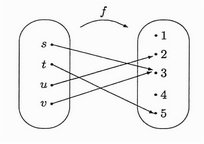
\includegraphics[scale=0.55]{HibCollArrow.jpg}
\end{center}

%---------------------------------------%
\subsection*{Question 6}
%2002 Question 7
Let $\mathcal{S}$ be a set and let $\mathcal{R}$ be a relation on $\mathcal{S}$
Explain what it means to say that $\mathcal{R}$ is

\begin{itemize}
	\item[(i)] reflexive
	\item[(ii)] symmetrix
	\item[(iii)] anti-symmetric
	\item[(iv)] Transitive
\end{itemize}


\subsection*{Question 10}

(a) Given the following adjacency matrices A and B where
%A =
%
%1 0 1
%0 1 2
%1 2 0
%
% ,B =
%
%1 2 0
%2 0 1
%0 1 1

%MAKE NO

%--------------------------------------------%

(i) Say whether or not the graphs they represent are isomorphic.
(ii) Calculate A2 and A4 and say what information each gives about the graph
corresponding to A. [6]
(b) (i) Write down the augmented matrix for the following system of equations.

\[2x + y - z = 2\]
\[x - y + z = 4\]
\[x + 2y + 2z = 10\]
(ii) Use Gaussian elimination to solve the system. [4]










\end{document}
